%Correct the file name.
%X: book number
%Y: part number
%ZZZ: page number in three digits. So page 3 would be 003.

\documentclass[11pt]{amsbook}

\usepackage{../HBSuerDemir}	% ------------------------


\begin{document}

% ++++++++++++++++++++++++++++++++++++++
\hPage{b2p1/145}
% ++++++++++++++++++++++++++++++++++++++

\begin{equation*}
	c_1u_1+\cdots+c_nu_n=0,		(c_i\epsilon\mathbb{R})
\end{equation*}
one has
\begin{equation*}
	c_1(u_n,\cdots,u_{1n})+\cdots+c_n(u_{n1},\cdots,u_{nn}) = 0
\end{equation*}
or
\begin{equation*}
	(c_1u_{11}+\cdots+c_nu_{n1},\cdots,c_nu_{11}+\cdots+c_nu_{nn}) = 0
\end{equation*}
implying the homogeneous square system

\begin{center}
	\begin{tabular}{lllll}
		$u_{11}c_1$ & $+\cdots+$ & $u_{n1}c_n$ & $=$ & $0$ \\
		$\vdots$ & & $\vdots$ && $\vdots$ \\
		$u_{1n}c_n1$ & $+\cdots+$ & $u_{nn}c_n$ & $=$ & $0$
	\end{tabular}
\end{center}
of linear equations in the unknowns $c_1,\cdots,c_n$ of which the determinant is $D=det|u_{ij}|$.

If $D\neq0$, the system admits solution other tfian the trivial one, meaning that not all $c$'s are zero, and the vectors are linearly dependent.

\begin{enumerate}
	\item[2.] $\mathbb{R}^n$ contains the unit vectors
\end{enumerate}
\begin{equation*}
	e_1=(1,0,\cdots,0),\cdots,e_n=(0,\cdots,0,1)
\end{equation*}
which are linearly independent since $det|u_{ij}|$ is $|I_n| = 1 \neq 0$.

\begin{enumerate}
	\item[3.] Let $u_1,\cdots,u_n,u_{n+1}$ be non zero vectors in $\mathbb{R}^n$.
\end{enumerate}
The theorem is proved if n of them, say $u_1, \cdots,u_n$ are linearly dependent, in which case $u_1, \cdots,u_n,u_{n+1}$ are linearly dependent.

Let the $u_1,\cdots,u_n$ be linearly independent. It will then suffice to prove that $u=u_{n+1}$ is a linear combination of $u_1,\cdots,u_n$:
\begin{equation*}
	c_1u_1+\cdots+c_nu_n=u
\end{equation*}
% =======================================================
\end{document}  

%==== templates ====

%==== environments ====

%\begin{figure}[htb]
%	\centering
%	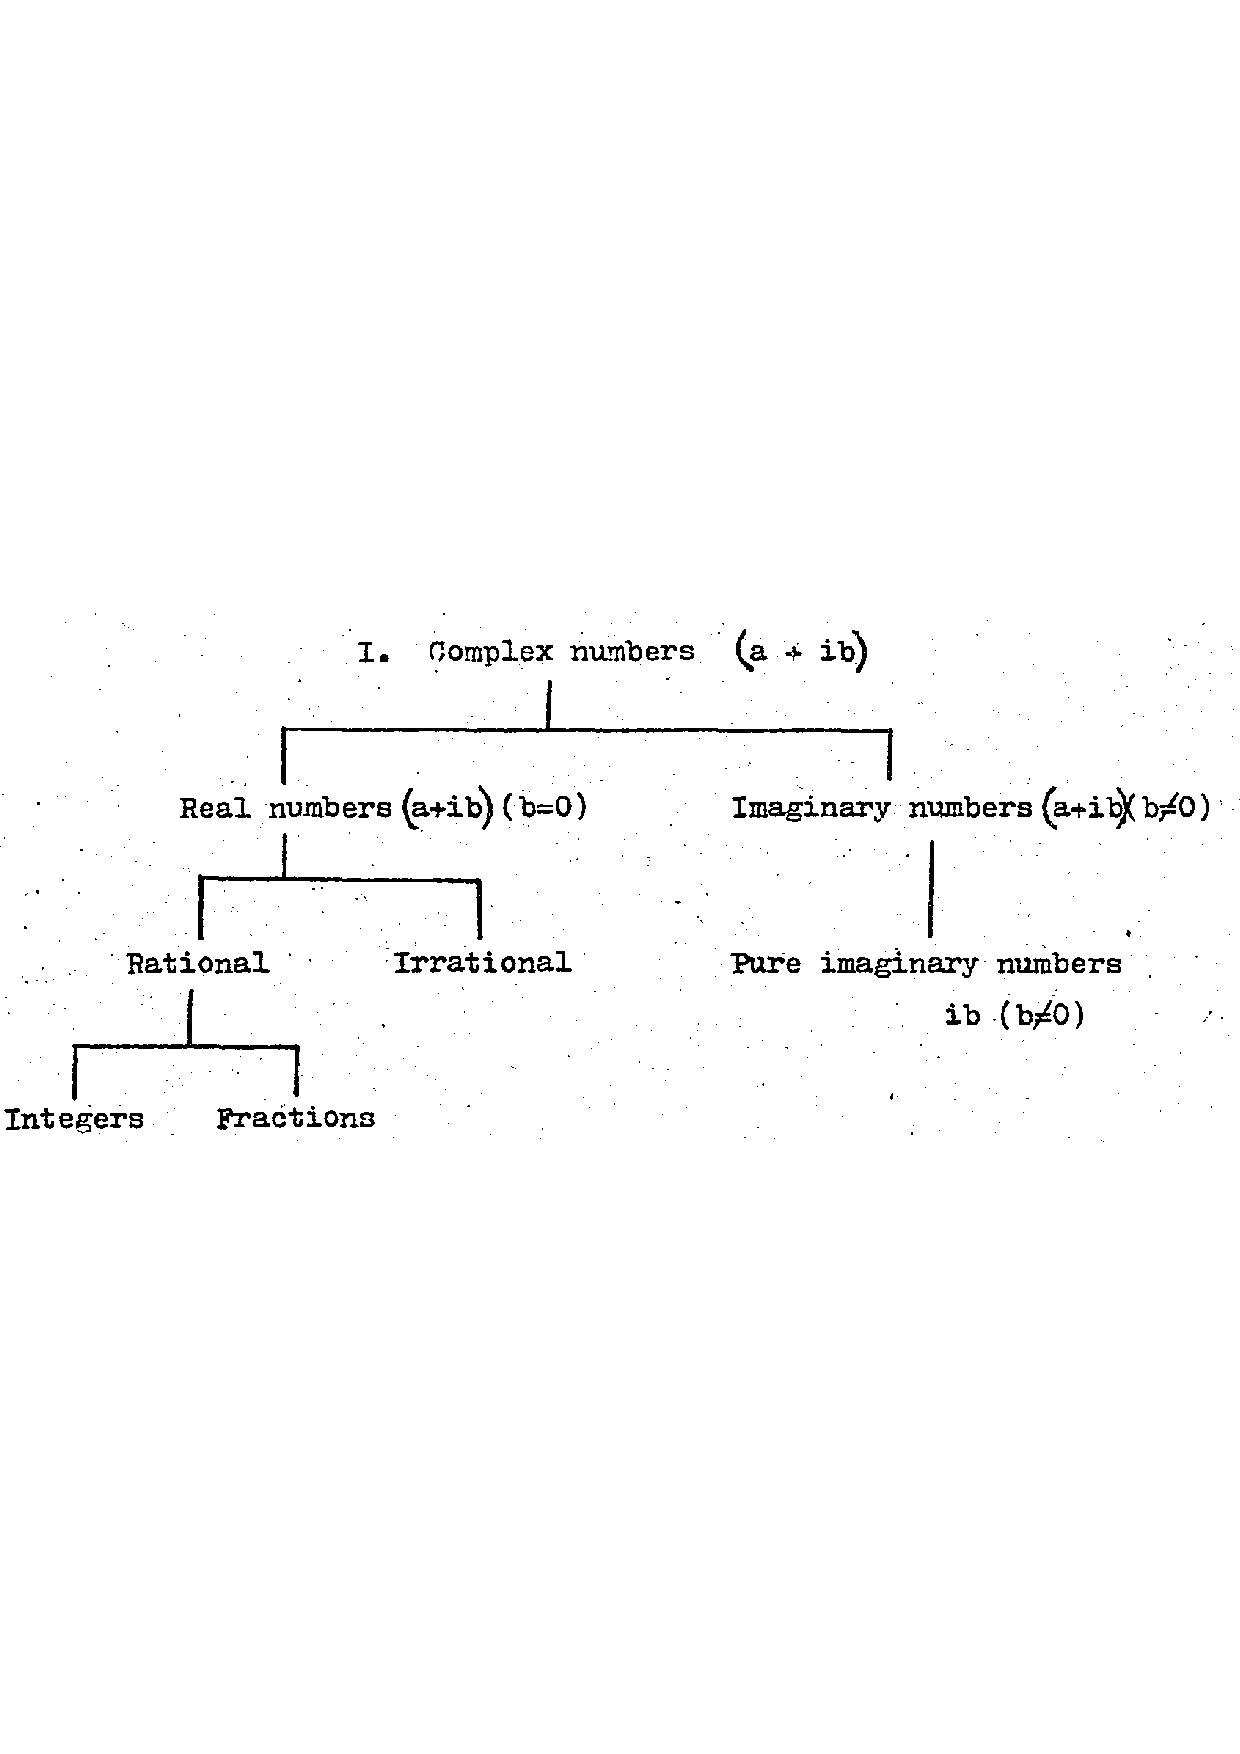
\includegraphics[width=0.9\textwidth]{images/SD-1-1p15A}
%	\caption{Classification of complex numbers}
%	\label{fig:classificationOfComplexNumbersA}
%\end{figure}

%\begin{center}
%\begin{tabular}{cc}
%\end{tabular}
%\end{center}

%\begin{exmp}
%\begin{hSolution}
%\end{hSolution}
%\end{exmp}

%\begin{hEnumerateAlpha}
%\end{hEnumerateAlpha}

%\begin{hEnumerateRoman}
%\end{hEnumerateRoman}

%$
%\begin{bmatrix}
%\end{bmatrix}
%$

%\frac{aaaa}{bbb}
%\frac{a_{n}}{b_{n}}
%\left( aaaa \right)
%\Longrightarrow

%\begin{multicols}{2}
%	bb
%\columnbreak
%	aa
%\end{multicols}
